\chapter{ผลการศึกษา}\label{ch:results}

\paragraph{}
บทนี้จะนำเสนอผลการดำเนินงานของโครงการวิจัย KGs-Augmented Testsuite Generator Framework โดยจะแสดงให้เห็นว่ากรอบการทำงานที่พัฒนาขึ้นสามารถบรรลุวัตถุประสงค์ที่ตั้งไว้ได้อย่างไร พร้อมทั้งนำเสนอตัวอย่างผลลัพธ์ที่ได้จากระบบ การเปรียบเทียบกระบวนการก่อนและหลังการพัฒนา และรายงานผลการประเมินประสิทธิภาพของกรอบการทำงาน

\section{ผลการดำเนินงานตามวัตถุประสงค์}\label{sec:}

\paragraph{}
กรอบการทำงานที่พัฒนาขึ้นสามารถดำเนินงานได้สำเร็จและสอดคล้องกับวัตถุประสงค์หลักทั้ง 3 ข้อที่ได้ตั้งไว้ ดังนี้

\begin{enumerate}
    \item \textbf{วัตถุประสงค์ข้อที่ 1: พัฒนากรอบการสร้างชุดทดสอบที่น่าเชื่อถือ (KGs-Augmented Testsuite Generator)}
    \begin{itemize}
        \item \textbf{ผลการดำเนินงาน:} ประสบความสำเร็จในการพัฒนากรอบการทำงานที่สมบูรณ์ ซึ่งสามารถสกัดข้อมูลจากรายงานอุบัติเหตุ (Unstructured Text) ด้วย Schema-guided LLM และสร้างเป็น Knowledge Graph (KG) เพื่อใช้เป็นรากฐานเชิงความหมายของข้อมูลได้จริง ซึ่งแสดงให้เห็นถึงการบูรณาการเทคโนโลยี LLM และ KG เข้าด้วยกันอย่างเป็นระบบ
    \end{itemize}

    \item \textbf{วัตถุประสงค์ข้อที่ 2: เพิ่มประสิทธิภาพการค้นพบ Edge-Case ด้วยการบูรณาการ ODD}
    \begin{itemize}
        \item \textbf{ผลการดำเนินงาน:} บรรลุวัตถุประสงค์หลักของงานวิจัย โดยได้พัฒนากลไกการค้นหา Edge-Case ที่มีประสิทธิภาพผ่านการใช้ \textbf{ODD Modular} และเทคนิค \textbf{Query Rotation} ผลลัพธ์จากการดำเนินงานสามารถจำแนกรายงานอุบัติเหตุจริงจำนวน 318 กรณีศึกษา ออกเป็นกลุ่ม ODD Modular ที่มีความหมายได้ถึง 21 กลุ่ม ซึ่งเป็นการยืนยันว่ากรอบการทำงานสามารถกรองและมุ่งเป้าการสร้างสถานการณ์ไปยังขอบเขตที่ท้าทายระบบได้อย่างเป็นรูปธรรม ช่วยลดการสร้างเหตุการณ์ที่ไม่จำเป็นลงได้อย่างมีนัยสำคัญ
    \end{itemize}

    \item \textbf{วัตถุประสงค์ข้อที่ 3: สร้างผลลัพธ์ที่มีโครงสร้างและเป็นมาตรฐาน}
    \begin{itemize}
        \item \textbf{ผลการดำเนินงาน:} กรอบการทำงานสามารถสร้างผลลัพธ์สุดท้ายในรูปแบบของชุดพารามิเตอร์ (Parameter Set) ที่มีโครงสร้างสมบูรณ์และถูกต้องตามหลักเหตุผล ซึ่งพร้อมสำหรับนำไปใช้งานร่วมกับ Scenario Template ในมาตรฐานอุตสาหกรรมอย่าง ASAM OpenSCENARIO ได้ทันที ดังที่ได้อธิบายไว้ในขั้นตอนวิธี (บทที่ 4)
    \end{itemize}
\end{enumerate}

\section{ตัวอย่างผลลัพธ์}

\subsection{ผลการจำแนกประเภทอุบัติเหตุด้วย ODD Modular}
\paragraph{}
หัวใจสำคัญของกรอบการทำงานคือความสามารถในการจัดหมวดหมู่สถานการณ์อุบัติเหตุตามกลุ่ม ODD Modular ที่กำหนดไว้ล่วงหน้า จากการประมวลผลรายงานอุบัติเหตุทั้งหมด 318 กรณีศึกษา ระบบสามารถจำแนกและนับจำนวนเคสที่เข้าข่ายแต่ละกลุ่มได้อย่างแม่นยำ ดังแสดงในตารางที่~\ref{tab:odd_modular_results} ซึ่งแสดงให้เห็นถึงการกระจายตัวของสถานการณ์ประเภทต่างๆ

\begin{table}[htbp]
    \centering
    \caption{ผลการจำแนกประเภทอุบัติเหตุ 318 กรณีศึกษาตามกลุ่ม ODD Modular ทั้ง 21 กลุ่ม}
    \label{tab:odd_modular_distribution}
    \begin{tabular}{|l|c|c|}
        \hline
        \rowcolor{gray!20} \textbf{ODD Modular Group} & \textbf{Percentage (\%)} & \textbf{Case Count} \\
        \hline
        \multicolumn{3}{|c|}{\textbf{1. Intersections / Junctions (I) - High Complexity}} \\
        \hline
        I-1: Signalized Conflict & 3.91 & 12 \\
        I-2: Unsignalized Left-Turn & 9.09 & 29 \\
        I-3: Roundabout Conflict & 5.42 & 17 \\
        I-4: Intersection Queue Mgmt & 4.25 & 14 \\
        I-5: Crosswalk Pedestrian Conflict & 3.07 & 10 \\
        I-6: Four-Way Stop Misinterpretation & 13.70 & 44 \\
        I-7: Grade/Curvature Intersection & 5.06 & 16 \\
        \hline
        \multicolumn{3}{|c|}{\textbf{2. Traffic Maneuvers (T) - High Frequency}} \\
        \hline
        T-1: Rear-End Collision & 6.62 & 21 \\
        T-2: Aggressive Cut-In & 5.38 & 17 \\
        T-3: Unsafe Lane Change & 2.88 & 9 \\
        T-4: Following Too Closely & 2.55 & 8 \\
        T-5: Wrong-Way Driving & 7.52 & 24 \\
        T-6: Unexpected Lane Departure & 7.95 & 25 \\
        T-7: Cyclist/Motorcyclist Close Pass & 2.94 & 9 \\
        \hline
        \multicolumn{3}{|c|}{\textbf{3. Adverse Environment / Structure (E) - High Severity}} \\
        \hline
        E-1: Heavy Rainfall / Low Friction & 4.00 & 13 \\
        E-2: Nighttime / Poor Illumination & 2.74 & 9 \\
        E-3: Sun Glare / Low Sun Angle & 3.49 & 11 \\
        E-4: Construction Zone Conflict & 2.28 & 7 \\
        E-5: Fog / Dust Storm & 3.33 & 11 \\
        E-6: Road Obstacle / Debris & 1.69 & 5 \\
        E-7: Toll/Entrance Gate Merge & 2.13 & 7 \\
        \hline
    \end{tabular}
\end{table}

\subsection{กรณีศึกษา C00013: Intersection Signalized Conflict}
\paragraph{}
เพื่อแสดงให้เห็นภาพการทำงานตั้งแต่ต้นจนจบ ขอนำเสนอกรณีศึกษา C00013 ซึ่งเป็นอุบัติเหตุ ณ ทางแยกที่มีสัญญาณไฟ กรอบการทำงานได้สกัดข้อมูลจากรายงานที่เป็นข้อความ และสร้างเป็นชุดพารามิเตอร์ที่มีโครงสร้างดังรูปที่~\ref{fig:c00013_features} ซึ่งพารามิเตอร์เหล่านี้ถูกนำไปใช้สร้างสถานการณ์จำลองที่สมจริงได้ในท้ายที่สุด ดังแสดงในรูปที่~\ref{fig:c00013_simulation}

\begin{figure}[htbp]
    \centering
    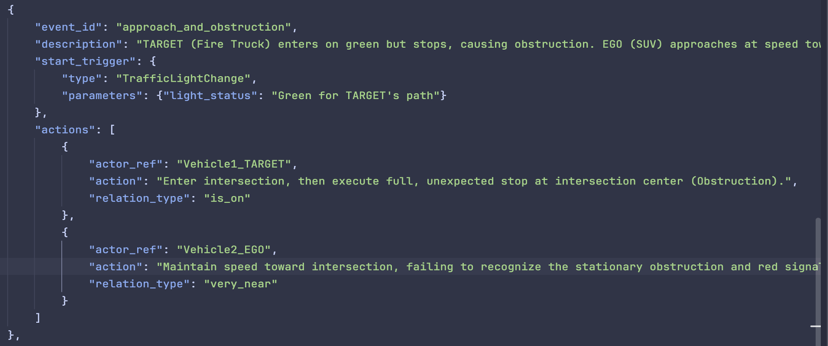
\includegraphics[width=0.9\textwidth]{images/c00013_extracted_features}
    \caption{ตัวอย่างชุดพารามิเตอร์ที่มีโครงสร้างซึ่งถูกสกัดจากรายงานอุบัติเหตุ C00013}
    \label{fig:c00013_features}
\end{figure}

\begin{figure}[htbp]
    \centering
    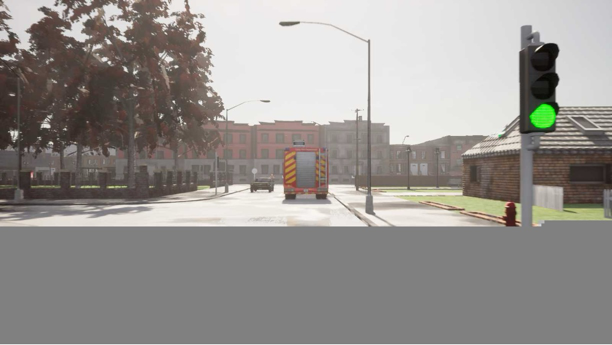
\includegraphics[width=0.49\textwidth]{images/c00013_sim_front}
    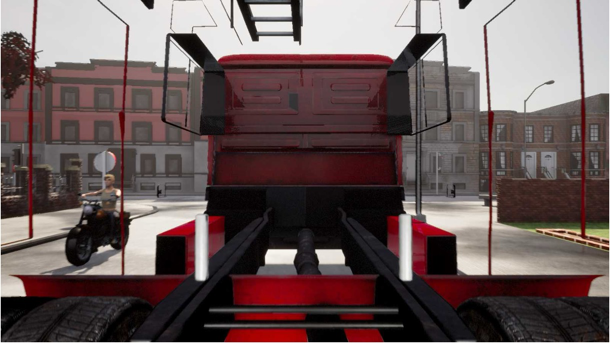
\includegraphics[width=0.49\textwidth]{images/c00013_sim_front_col}
    \caption{ภาพจากสถานการณ์จำลองของกรณีศึกษา C00013 ที่สร้างขึ้นจากพารามิเตอร์ของระบบ (ซ้าย: มุมมองด้านหน้า, ขวา: มุมมองด้านหน้าขณะชน)}
    \label{fig:c00013_simulation}
\end{figure}

\section{การเปรียบเทียบก่อนและหลังการพัฒนา}
\paragraph{}
การนำกรอบการทำงาน KGs-Augmented Testsuite Generator มาใช้ได้เปลี่ยนแปลงกระบวนการสร้างชุดทดสอบจากการพยายามแบบไร้ทิศทางไปสู่กระบวนการที่เป็นระบบและมุ่งเน้นเป้าหมายอย่างชัดเจน ดังนี้

\begin{itemize}
    \item \textbf{ก่อนการพัฒนา:} การใช้ LLM โดยตรงเพื่อสร้างสถานการณ์จากรายงานอุบัติเหตุมีลักษณะเป็นการ "สุ่ม" ซึ่งต้องสร้างสถานการณ์ที่ไม่ท้าทายระบบ (Normal Safe Scenarios) จำนวนมากเพื่อที่จะพบ Edge-Case ที่มีความหมายเพียงไม่กี่กรณี ทำให้มีประสิทธิภาพการค้นพบกรณีขอบเขต (Edge-Case Discovery Efficiency) ที่ต่ำ และสิ้นเปลืองทรัพยากรอย่างมาก

    \item \textbf{หลังการพัฒนา:} กรอบการทำงานใหม่ใช้ KG เป็นฐานความรู้และใช้ ODD Modular เป็นตัวกรอง ทำให้กระบวนการสร้างสถานการณ์มีเป้าหมายที่ชัดเจน (Goal-Oriented) โดยมุ่งเน้นไปที่การค้นหาเคสที่ตรงตามเงื่อนไขความเสี่ยงที่กำหนดไว้เท่านั้น ส่งผลให้ ประสิทธิภาพการค้นพบกรณีขอบเขตสูงขึ้นอย่างมีนัยสำคัญ และลดจำนวนครั้งในการสร้างเหตุการณ์ซ้ำซ้อนลงได้
\end{itemize}

\section{การประเมินผล}
\paragraph{}
เพื่อประเมินคุณภาพและความสมจริงของผลลัพธ์ ได้มีการใช้แนวคิดการประเมินเชิงเทคนิคที่เรียกว่า Scenario Completeness Score หรือ R-score (Realism Score) ซึ่งเป็นการวัดความคล้ายคลึงกันระหว่าง Scene Graph ของสถานการณ์ในอุบัติเหตุจริง กับ Scene Graph ที่สร้างขึ้นจากพารามิเตอร์ของกรอบการทำงาน

\paragraph{}
ผลการประเมินเบื้องต้นพบว่าค่า R-score มีความแตกต่างกันไปในแต่ละ ODD Modular ซึ่งชี้ให้เห็นว่ากรอบการทำงานมีความสามารถในการสร้างสถานการณ์ที่มีความซับซ้อนแตกต่างกันได้ดี ดังแสดงในตารางที่~\ref{tab:r_score_results}

\begin{table}[htbp]
    \centering
    \caption{ตัวอย่างผลการประเมิน R-score ในกลุ่ม ODD Modular ต่างๆ}
    \label{tab:r_score_results}
    \begin{tabular}{|l|c|}
        \hline
        \rowcolor{gray!20} \textbf{ODD Modular Group} & \textbf{Average R-score} \\
        \hline
        T-1: Rear-End Collision & \textbf{0.9577} (สูง) \\
        \hline
        E-6: Road Obstacle - Debris & \textbf{0.6305} (ต่ำ) \\
        \hline
    \end{tabular}
\end{table}

\paragraph{}
จากตาราง ผลการประเมินชี้ว่าสถานการณ์ที่มีปฏิสัมพันธ์ระหว่างยานพาหนะที่ไม่ซับซ้อน เช่น "การชนท้าย" (Rear-End Collision) สามารถสร้างได้อย่างสมจริงและได้ R-score ที่สูง ในขณะที่สถานการณ์ที่เกี่ยวข้องกับวัตถุบนถนนแบบสุ่ม เช่น "สิ่งกีดขวาง" (Road Obstacle) ยังคงมีความท้าทายในการสกัดข้อมูลและสร้างให้สมจริง ซึ่งเป็นแนวทางสำหรับการพัฒนาต่อไปในอนาคต